
 % ------------------------------------------------------------------------
% ------------------------------------------------------------------------
% Modelo de Trabalho Academico (tese de doutorado, dissertacao de
% mestrado e trabalhos monograficos em geral) em conformidade com 
% ABNT NBR 14724:2011: Informacao e documentacao - Trabalhos academicos -
% UNIVERSIDADE FEDERAL FLUMINENSE
% ------------------------------------------------------------------------
% ------------------------------------------------------------------------

\documentclass[
	% -- opções da classe memoir --
	12pt,				% tamanho da fonte
	openright,			% capítulos começam em pág ímpar (insere página vazia caso preciso)
	oneside,			% para impressão em recto e verso. Oposto a oneside
	a4paper,			% tamanho do papel. 
	% -- opções da classe abntex2 --
	%chapter=TITLE,		% títulos de capítulos convertidos em letras maiúsculas
	%section=TITLE,		% títulos de seções convertidos em letras maiúsculas
	%subsection=TITLE,	% títulos de subseções convertidos em letras maiúsculas
	%subsubsection=TITLE,% títulos de subsubseções convertidos em letras maiúsculas
	% -- opções do pacote babel --
	english,			% idioma adicional para hifenização
	french,				% idioma adicional para hifenização
	spanish,			% idioma adicional para hifenização
	brazil				% o último idioma é o principal do documento
	]{abntex2}

% ----
\usepackage{Template_v01}			% carrega os arquivos de formatação		
\usepackage{amsmath}
\renewcommand\chapternumberline[1]{\numberline{#1}}

%Pacote Adicionado - Pode Retirar depois

%Fim do Pacote Adicionado

\pagestyle{myheadings}
      
\providetoggle{TCC} 
\providetoggle{Dissertacao}
\providetoggle{Tese}
% seleciona modelo para graduação ou pós-graduação (TCC, Dissertacao, Tese)
\settoggle{TCC}{true}
\settoggle{Dissertacao}{false}
\settoggle{Tese}{false}

% Informações de dados para CAPA e FOLHA DE ROSTO
% ---
\titulo{105Quantificação do efeito de tumores  superficiais e profundos sobre a  
temperatura da pele}
\autor{AUTOR, INICIAIS MAIÚSCULAS E RESTANTE MINÚSCULO}
\local{Niterói, RJ}
\data{DATA}
\orientador{ORIENTADOR}
\instituicao{%
  UNIVERSIDADE FEDERAL FLUMINENSE
  \par
  ESCOLA DE ENGENHARIA
  \par
  \iftoggle{TCC}{PROGRAMA DE GRADUAÇÃO EM ENGENHARIA MECÂNICA}{}
  \iftoggle{Dissertacao}{PROGRAMA FRANCISCO EDUARDO MOURÃO SABOYA DE PÓS-GRADUAÇÃO EM ENGENHARIA MECÂNICA}{}
  \iftoggle{Tese}{PROGRAMA FRANCISCO EDUARDO MOURÃO SABOYA DE PÓS-GRADUAÇÃO EM ENGENHARIA MECÂNICA}{}}

% O preambulo deve conter o tipo do trabalho, o objetivo, 
% o nome da instituição e a área de concentração 
\iftoggle{TCC}{
	\tipotrabalho{Trabalho de Conclusão do Curso}
	\preambulo{ Trabalho de Conclusão de Curso
	apresentado ao Curso de Engenharia Mecânica da
	Universidade Federal Fluminense, como requisito
	parcial para obtenção do grau de Engenheiro
	Mecânico.}
	}{}
\iftoggle{Dissertacao}{
	\tipotrabalho{Dissertação}
	\preambulo{Dissertação apresentada
ao Programa de Pós-graduação em Engenharia Mecânica
da Universidade Federal Fluminense, como parte dos requisitos 
para a obtenção do título de Mestre em Ciências 
em Engenharia Mecânica.}
	}{}
\iftoggle{Tese}{
	\tipotrabalho{Tese}
	\preambulo{Tese apresentada ao Programa de 
Pós-graduação em Engenharia Mecânica da Universidade 
Federal Fluminense, como parte dos requisitos para a obtenção 
do título de Doutor em Ciências em Engenharia Mecânica.}
	}{}
% ---

% ---
% Configurações de aparência do PDF final

% informações do PDF
\makeatletter
\hypersetup{
     		%pagebackref=true,
		pdftitle={\@title}, 
		pdfauthor={\@author},
    		pdfsubject={\imprimirpreambulo},
	   	pdfcreator={LaTeX with abnTeX2},
		pdfkeywords={abnt}{latex}{abntex}{abntex2}{trabalho acadêmico}, 
		colorlinks=true,       		% false: boxed links; true: colored links
    		linkcolor=black,          	% color of internal links
    		citecolor=black,        		% color of links to bibliography
    		filecolor=magenta,      		% color of file links
		urlcolor=blue,
		bookmarksdepth=4
}
\makeatother
% --- 

% ---
% Posiciona figuras e tabelas no topo da página quando adicionadas sozinhas
% em um página em branco. Ver https://github.com/abntex/abntex2/issues/170
\makeatletter
\setlength{\@fptop}{5pt} % Set distance from top of page to first float
\makeatother
% ---

% ---
% Possibilita criação de Quadros e Lista de quadros.
% Ver https://github.com/abntex/abntex2/issues/176
%
\newcommand{\quadroname}{Quadro}
\newcommand{\listofquadrosname}{Lista de quadros}

\newfloat[chapter]{quadro}{loq}{\quadroname}
\newlistof{listofquadros}{loq}{\listofquadrosname}
\newlistentry{quadro}{loq}{0}

% configurações para atender às regras da ABNT
\setfloatadjustment{quadro}{\centering}
\counterwithout{quadro}{chapter}
\renewcommand{\cftquadroname}{\quadroname\space} 
\renewcommand*{\cftquadroaftersnum}{\hfill--\hfill}

\setfloatlocations{quadro}{hbtp} % Ver https://github.com/abntex/abntex2/issues/176
% ---

% --- 
% Espaçamentos entre linhas e parágrafos 
% --- 

% O tamanho do parágrafo é dado por:
\setlength{\parindent}{1.3cm}

% Controle do espaçamento entre um parágrafo e outro:
\setlength{\parskip}{0.2cm}  % tente também \onelineskip

%\renewcommand{\baselinestretch}{2.0}
% ---
% compila o indice
% ---
\makeindex
% ---

% ----
% Início do documento
% ----


\begin{document}




% Seleciona o idioma do documento (conforme pacotes do babel)
%\selectlanguage{english}
\selectlanguage{brazil}

% Retira espaço extra obsoleto entre as frases.
\frenchspacing 

% ----------------------------------------------------------
% ELEMENTOS PRÉ-TEXTUAIS
% ----------------------------------------------------------
% \pretextual

% ---
% Capa
% ---
\imprimircapa
% ---

% ---
% Folha de rosto
% (o * indica que haverá a ficha bibliográfica)
% ---
\imprimirfolhaderosto*
% ---

% ---
% Inserir a ficha bibliografica
% ---

% Isto é um exemplo de Ficha Catalográfica, ou ``Dados internacionais de
% catalogação-na-publicação''. Você pode utilizar este modelo como referência. 
% Porém, provavelmente a biblioteca da sua universidade lhe fornecerá um PDF
% com a ficha catalográfica definitiva após a defesa do trabalho. Quando estiver
% com o documento, salve-o como PDF no diretório do seu projeto e substitua todo
% o conteúdo de implementação deste arquivo pelo comando abaixo:
%
 \begin{fichacatalografica}
     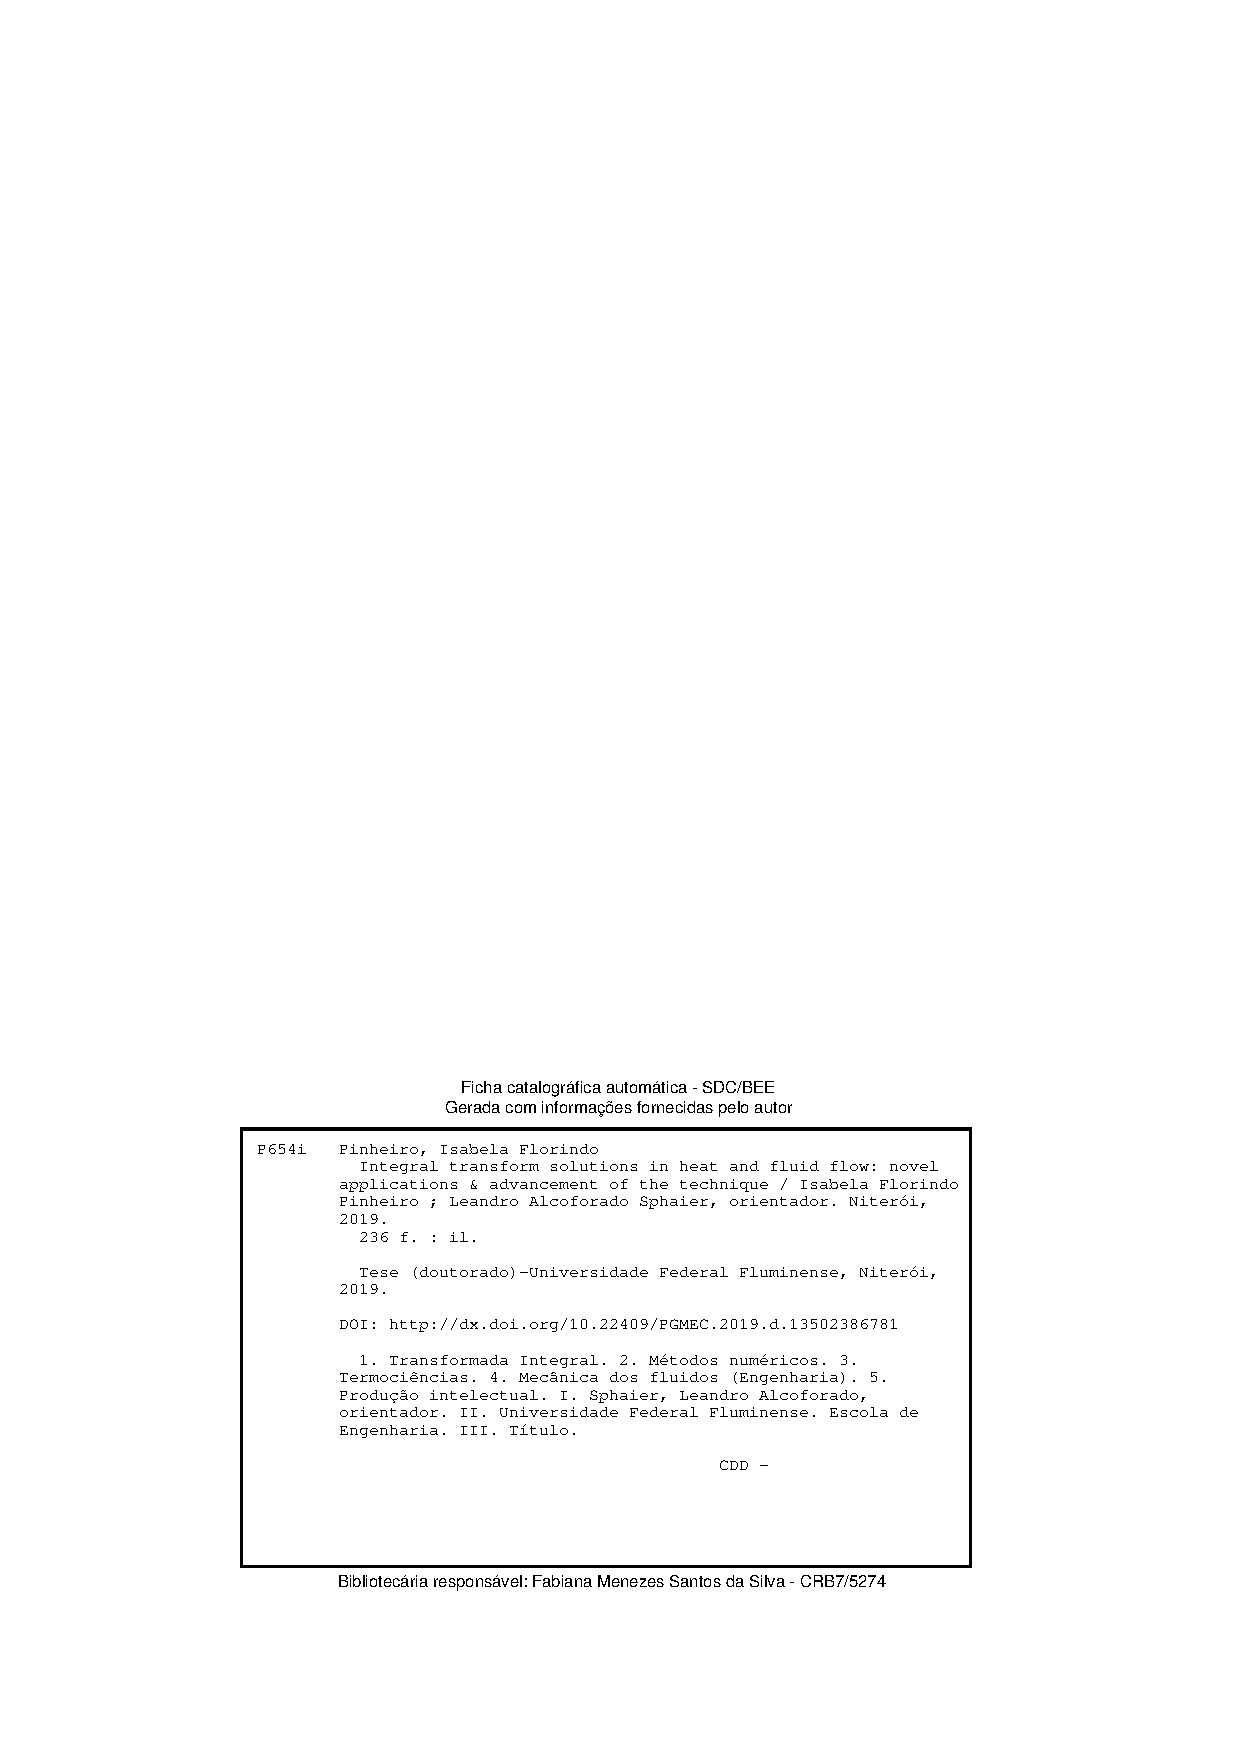
\includepdf{ficha.pdf}
 \end{fichacatalografica}


% ---

% ---
% Inserir folha de aprovação
% ---

% Isto é um exemplo de Folha de aprovação, elemento obrigatório da NBR
% 14724/2011 (seção 4.2.1.3). Você pode utilizar este modelo até a aprovação
% do trabalho. Após isso, substitua todo o conteúdo deste arquivo por uma
% imagem da página assinada pela banca com o comando abaixo:
%
%\begin{folhadeaprovacao}
% \includepdf{folhadeaprovacaofinal.pdf}
%\end{folhadeaprovacao}
%
	\begin{folhadeaprovacao}
	
	  \begin{center}
	    {\ABNTEXchapterfont\large\imprimirautor}
	
	    \vspace*{\fill}\vspace*{\fill}
	    \begin{center}
	      \ABNTEXchapterfont\bfseries\Large\imprimirtitulo
	    \end{center}
	    \vspace*{\fill}
	    
	    \hspace{.45\textwidth}
	    \begin{minipage}{.5\textwidth}
	    \DoubleSpacing
	        \imprimirpreambulo
	    \end{minipage}%
	    \vspace*{\fill}
	   \end{center}
	     
	   Grau: 
	        
	   Aprovado em \imprimirdata
	   
	   \begin{center}
	   BANCA EXAMINADORA
	   \end{center}
	   
	   \assinatura{\textbf{\imprimirorientador} \\ Orientador \\[1.5em] } 
	   \assinatura{\textbf{Prof. DSc César Cunha Pacheco} \\[1.5em] }
	   \assinatura{\textbf{Eng. Matheus Coutinho Constantino } \\[1.5em] } %Dependendo da quantidade de membros da banca, regular os espaços entre cada assinatura
	   %\assinatura{\textbf{Professor} \\ Convidado 3}
	   %\assinatura{\textbf{Professor} \\ Convidado 4}
      
   \begin{center}
   \vspace*{0.5cm}
  {\large\imprimirlocal}
  \par
  {\large\imprimirdata}
  \vspace*{1cm}
  \end{center}
  
\end{folhadeaprovacao}
% ---
% ---
% Dedicatória
% ---
\begin{dedicatoria}
   \vspace*{\fill}
   \centering
   \noindent
   \vspace*{0.75\textheight}
   \begin{flushright}
    \DoubleSpacing
   \textit{ Dedicatória. \\
   	Colocar em página ímpar. \\
   	Esta seção é opcional.} 
	\end{flushright}
	\vspace*{\fill}
\end{dedicatoria}
% ---
\textual 
\frontmatter
% ---
% Agradecimentos
% ---
\begin{agradecimentos}
\addcontentsline{toc}{chapter}{Agradecimentos}
Agradecimentos

Colocar em página ímpar.

Esta seção é opcional.

Citar agência de fomento, se houver.


\end{agradecimentos}
% ---

% ---
% Epígrafe
% ---
\begin{epigrafe}
    \vspace*{\fill}
	\begin{flushright}
		\textit{Epígrafe}
	\end{flushright}
\end{epigrafe}
% ---

% ---
% RESUMOS
% ---

% resumo em português
\setlength{\absparsep}{18pt} % ajusta o espaçamento dos parágrafos do resumo
\begin{resumo}
\addcontentsline{toc}{chapter}{Resumo}
Sumarização do trabalho realizado, sem apresentar motivação, revisão da literatura e revisão teórica. Focar no trabalho desenvolvido, métodos, resultados, etc., e sumarizar conclusões.
\textbf{Palavras-chave:} Palavra-chave 1, palavra-chave 2, palavra-chave 3.

\end{resumo}

% resumo em inglês
\begin{resumo}[Abstract]
\addcontentsline{toc}{chapter}{Abstract}
 \begin{otherlanguage*}{english}
	
	
	Colocar em página ímpar

   \vspace{\onelineskip}
 
   \noindent 
   \textbf{Keywords}
 \end{otherlanguage*}
\end{resumo}


% ---

% ---
% inserir lista de ilustrações
% ---
\pdfbookmark[0]{\listfigurename}{lof}
\listoffigures*
\addcontentsline{toc}{chapter}{Lista de Ilustrações}
\cleardoublepage
% ---

% ---
% inserir lista de quadros
% ---


% ---
% inserir lista de tabelas
% ---
\pdfbookmark[0]{\listtablename}{lot}
\listoftables*
\addcontentsline{toc}{chapter}{Lista de tabelas}
\cleardoublepage
% ---

% ---
% inserir lista de abreviaturas e siglas
% ---
\begin{siglas}
\addcontentsline{toc}{chapter}{Lista de abreviaturas e siglas}
  \item[COP] \textit{Coefficient of performance}
  \item[EOS] \textit{Equation of state}
  \item[GWP] \textit{Global Warming Potential}
  \item[IEA] \textit{International Energy Agency}
  \item[IIAR] \textit{International Institute of Ammonia Refrigeration}
  \item[ODP] \textit{Ozone depletion potential}
  \item[PR-EOS] \textit{Peng-Robinson Equation of state}
\end{siglas}
% ---

% ---
% inserir lista de símbolos
%usar [r] para letras romanas, [g] para letras gregas e [s] para subíndices
% ---
\mbox{}

\nomenclature[r]{$\dot{m}$}{Vazão mássica}
\nomenclature[g]{$\rho$}{Densidade molar}
\nomenclature[s]{$i$}{Estado ou ponto $i$}
\printnomenclature	
\pagebreak

\begin{simbolos}
\addcontentsline{toc}{chapter}{Lista de símbolos}
\item[$ \Gamma $] Letra grega Gama
\item[$ \Lambda $] Lambda
\item[$ \zeta $] Letra grega minúscula zeta
\item[$ \in $] Pertence
\end{simbolos}

% ---
% inserir o sumario
% ---
%\cftsetindents{section}{2em}{3em}
\pdfbookmark[0]{\contentsname}{toc}
\tableofcontents*
\cleardoublepage
% ---




% ----------------------------------------------------------
% ELEMENTOS TEXTUAIS
% ----------------------------------------------------------
\mainmatter

% ----------------------------------------------------------
% Introdução (exemplo de capítulo sem numeração, mas presente no Sumário)
% ----------------------------------------------------------
\chapter{INTRODUÇÃO}
% ----------------------------------------------------------
\section{Contextualizão}
 

Na atualidade, o cancêr é uma das efermidades que mais tem atingido as pessoas, tendo  mais de 18.1 milhões de casos diagnosticados e 9.6 milhões de mortes, somente em 2018. A estimativa é que em 2040, o número de casos anuais aumente em 50\%, ultrapassando os 27 milhões de casos. Essa estimativa tem uma alta variação, dependendo dos nível de desenvolvimento economico e social do país. Apesar de a maior parte dos casos diagnósticados serem em países com Índice de Desenvolvimento Humano(IDH) alto, conforme a Figura \ref{fig:casos-idh}, o aumento do número de casos de cancer em nações com baixo IDH é de 100\%, enquanto nas com IDH alto/muito alto é de aproximadamente 11%.



O câncer é a denominação dada ao conjunto de doenças que tem como característica comum a multiplicação descontrolada de células em um determinado tecido. Esse falta de controle advém de uma mutação no DNA da célula, que pode ocorrer devido a uma predisposição genética e/ou exposição a agentes carcinogênicos. 

Na atualidade, existem mais de 100 tipos de câncer descobertos. Para cada um deles existem diferentes tratamentos e técnicas de diagnosticos mais efetivas

\section{Objetivos}

\chapter{Revisão Bibliográfica}
O trabalho de \ref{} propós uma solução analítica para o modelo de Pennes em um
tecido com multiplas camadas e com a presença de um tumor. Utilizando uma técnica de
transformação integral, obteve-se distribuições de temperatura que estavam em acordo com
simulações computacionais previamente validadas.
\section{BIOTRANSFERÊNCIA DE CALOR}
\section{Termografia}
O Trabalho de (AGNELLI; BARREA; TURNER, 2011) é utilizou-se do métodos de
diferenças finitas de segunda ordem para resolver o modelo de Pennes em duas dimensões.
Através do uso de Algoritmo de Pattern Search foi possível obter informações cruciais sobre o
tumor, como seu tamanho e localização como a taxa de geração de calor devido ao metabolismo
do tumor.


\chapter{Modelagem Matemática}

\section{Modelagem}
Este trabalho  visa verificar a influência de diferentes configurações de tumores na superfície da pele. Considerou-se que o formato do antebraço de humano médio pode ser simplificado por um cilíndro maciço, dividido em três seções de diferentes diametros, representado pele, músculo e osso. As dimensões do cilíndro e de cada seção podem ser vistas na Figura \ref{fig:geometria} .

\begin{figure}[h!]
	\centering
	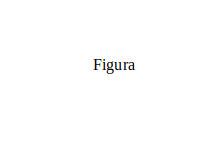
\includegraphics[width=0.6\textwidth]{Fig.png}
	\caption{ \label{fig:geometria}}
\end{figure}

Para a simplificação do problema, propôs-se as seguinte hipóteses:
\begin{itemize}
\item Regime Permanente
\item Problema Bidimensional, com axissimetria em torno do eixo Z.
\item Propriedades Físicas constantes e uniformes em cada tecido.
\item Tecidos Isotrópicos
\end{itemize}

O modelo de bio transferência de calor utilizado foi o Modelo de Pennes \ref{}, que apesar de sua simplicidade reproduz de maneira satisfatoria dados experimentais \ref{}. Esse modelo possui as seguintes variaveis:densidade do tecido $\rho$; condutividade térmica do tecido $k$; densidade do sangue $\rho_b$; calor específico do sangue a pressão constante $c_b$; taxa de perfusão sanguínea do tecido $w$; temperatura do sangue arterial $T_a$; temperatura do tecido analisado $T$; taxa de geração de calor metabolico por unidade de volume do tecido $Q_m$.

\begin{gather}
\rho c_p \frac{\partial T(r,z)}{\partial t} = \nabla \cdot [k(r) \nabla T(r,z)] + w_b \rho_b c_b[T_a-T(r,z)]+Q_m
\end{gather}

Utilizando as hipótese 1 e realizando a transformação para coordenadas cilíndricas, através da relação \ref{}, obtem-se a equação \ref{}.
\begin{gather}
\nabla \cdot [k(r) \nabla T(r,z)] =\frac{1}{r}\frac{\partial}{\partial r}k(r) r \frac{\partial T(r,z)}{\partial r}+\frac{\partial}{\partial z}k(r)\frac{\partial T(r,z)}{\partial z}
\end{gather}
\begin{gather}
\frac{1}{r}\frac{\partial}{\partial r}k r \frac{\partial T(r,z)}{\partial r}+\frac{\partial}{\partial z}k\frac{\partial T(r,z)}{\partial z} +\rho_b c_b w [T_a-T(r,z)] +Q_m=0 
\end{gather}

\subsection{Condições de Contorno}
A condição de contorno para a fronteira superior do problema(r=R) foi de troca de calor por convecção com o ambiente. Considerou-se que a perda de calor da pele por radiação com o ambiente é desprezível para a situação modelada ??. 

Para as fronteiras laterais, a condição de isolamento térmico foi utilizada. Essa condição de contorno é passível de ser utilizada caso a fronteira esteja distante o suficiente do elemento gerador de calor, neste caso o tumor.

Já para a fronteira inferior, a condição de isolamento térmico é a escolha natural, devido simetria térmica no centro do cilíndro (??).

\subsection{Volumes Finitos}
O método escolhido para a resolução numérica do modelo de biotranferência de calor
apresentado anteriormente foi o Método dos Volumes Finitos ??.

Esse método consiste na divisao do domínio em n volumes de controle discretos, onde é suposto que as variáveis de controle são constantes, e a resolução da equação de interesse dentro de cada volume.

Sendo P o volume de controle a ser estudado, os volumes W, E, N e S são os volumes vizinhos do mesmo. As fronteiras do volume P com os volumes adjacentes são nomeadas w, e, n e s, respectivamente.


\subsubsection{Discretização do Domínio}

A tipo de malha escolhida para o problema foi uniforme e retangular. Para manter os
volumes quadrados, a relação entre o número de volumes na direção r ena direção z obedece a fórmula 3.3.

Utilizou-se 3 diferentes malhas para verificar que a discretização não interferiu significativamente na resultado da simulação. 
De acordo com Celik o fator refinamento da malhar deve ser maior que 1.3.

\subsubsection{Integralização dos 
Termos}



\begin{figure}[h!]
	\centering
	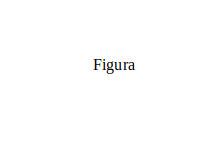
\includegraphics[width=0.6\textwidth]{Fig.png}
	\caption{ \label{fig:geometria}}
\end{figure}

Integrando a equação \ref{} ao longo do volume de controle de interesse:


\begin{gather}
\int_{\Delta V}\frac{1}{r}\frac{\partial}{\partial r}k r \frac{\partial T(r,z)}{\partial r}dV
+\int_{\Delta V} \frac{\partial}{\partial z}k\frac{\partial T(r,z)}{\partial z} dV
+\int_{\Delta V}\rho_b c_b w [T_a-T(r,z)]dV
+\int_{\Delta V} Q_m dV=0
\end{gather}

Dividiu-se a equação \ref{}, em 4 termos para facilitar a manipulação. 






\begin{gather}
\underbrace{\int_{s}^{n} \int_{e}^{w} \frac{1}{r}\frac{\partial}{\partial r}k r \frac{\partial T(r,z)}{\partial r}rdrdz}_\text{C1}    +\underbrace{\int_{s}^{n} \int_{e}^{w} \frac{\partial}{\partial z}k\frac{\partial T(r,z)}{\partial z} rdrdz}_\text{C2}    +\underbrace{\int_{s}^{n} \int_{e}^{w} \rho_b c_b w [T_a-T(r,z)]rdrdz}_\text{C3}+\underbrace{Q_m}_\text{C4}  =0
\end{gather}


A integralização do termo P1 é direta, Integrando-se, respectivamente, em r e em z e utilizando as relações \ref{} e \ref{} para obtem-se o resultado abaixo:

\begin{gather}
P1:\int_{s}^{n} \int_{e}^{w} \frac{1}{r}\frac{\partial}{\partial r}k r \frac{\partial T(r,z)}{\partial r}rdrdz=\int_{e}^{w} k r \frac{\partial T(r,z)}{\partial r} \biggr\rvert^{n}_{s} dz= 
\\
k r \frac{\partial T(r,z)}{\partial r} \biggr\rvert^{n}_{s} \Delta z= 
k_n r_n \frac{\partial T(r,z)}{\partial r}\biggr\rvert_{n}\Delta z-k_s r_s \frac{\partial T_s(r,z)}{\partial r}\biggr\rvert_{s}\Delta z
\end{gather} 

\begin{gather}
k_n r_n \frac{T_N-T_P}{\Delta r}\Delta z-k_s r_s  \frac{T_P-T_S}{\Delta r}\Delta z 
\end{gather} 

Para integral do termo P2, além do processo feito anteriormente, é necessário notar a relação \ref{} que é valida para malhas retangulares e uniformes.
\begin{gather}                                           
\frac{r^2}{2}\biggr\rvert^{n}_{s}=\frac{r_{n}^2}{2}-\frac{r_{s}^2}{2}=\frac{1}{2}\biggr(r_P+\frac{\Delta r}{2}\biggr)^2-\frac{1}{2}\biggr(r_P-\frac{\Delta r}{2}\biggr)^2=
\\
\frac{1}{2}\biggr(r_P^2+r_P\Delta r+\frac{\Delta r ^2}{4}\biggr)-\frac{1}{2}\biggr(r_P^2-r_P\Delta r+\frac{\Delta r ^2}{4}\biggr)=
r_P\Delta r
\end{gather}  

\begin{gather}                                           
P2:\int_{s}^{n} \int_{e}^{w}\frac{\partial}{\partial z}k \frac{\partial T(r,z)}{\partial z}rdrdz=\int_{s}^{n} r k \frac{\partial T(r,z)}{\partial z} \biggr\rvert^{w}_{e} dr=
\\
 \frac{r^2}{2}\biggr\rvert^{n}_{s} k \frac{\partial T(r,z)}{\partial r} \biggr\rvert^{w}_{e}=
r_P \Delta r k_w \frac{\partial T(r,z)}{\partial r} \biggr\rvert_{w} -r_P \Delta r k_e \frac{\partial T(r,z)}{\partial r} \biggr\rvert_{e}
\end{gather}
\begin{gather}
r_P \Delta r k_w \frac{T_W-T_P}{\Delta z} -r_P \Delta r k_e \frac{T_P-T_E}{\Delta z}
\end{gather}   
   
O termo P3, relacionado a transferência de calor devido a perfusão do sangue, pode ser integrado diretamente utilizando a equação \ref{} :
\begin{gather}                                           
P3:\int_{s}^{n} \int_{e}^{w} \rho_b c_b w [T_a-T(r,z)]rdrdz = \rho_b c_b w [T_a-T_P]\frac{r^2}{2}\biggr\rvert^{n}_{s}z\biggr\rvert^{w}_{e}\\ =\rho_b c_b w [T_a-T_P]r_P \Delta r\Delta z
\end{gather} 
Juntando os termos desenvolvidos, obtem-se a equação \ref{}. Como ela depende das derivada da temperatura no contorno do volume P, foi necessário aproximar os  gradientes de temperatura por diferenças finitas de primeira ordem, como pode ser visto nas equações \ref{}-\ref{}.
\begin{gather}
\label{eqn:semi_discre}
k_n r_n \frac{\partial T(r,z)}{\partial r}\biggr\rvert_{n}\Delta z-k_s r_s \frac{\partial T(r,z)}{\partial r}\biggr\rvert_{s}\Delta z
+
r_P \Delta r k_w \frac{\partial T(r,z)}{\partial z} \biggr\rvert_{w} -r_P \Delta r k_e \frac{\partial T(r,z)}{\partial z} \biggr\rvert_{e}
\\
=\rho_b c_b w [T_a-T_P]r_P \Delta r\Delta z
\end{gather}
\begin{gather}
\label{eqn:aprox_norte}
\frac{\partial T(r,z)}{\partial r}\biggr|_{n}=\frac{T_N-T_P}{\Delta r}
\end{gather}
\begin{gather}
\label{eqn:aprox_sul}
\frac{\partial T(r,z)}{\partial r}\biggr|_{s}=\frac{T_P-T_S}{\Delta r}
\end{gather}
\begin{gather}
\label{eqn:aprox_leste}
\frac{\partial T(r,z)}{\partial z}\biggr|_{e}=\frac{T_E-T_P}{\Delta z}
\end{gather}
\begin{gather}
\label{eqn:aprox_oeste}
\frac{\partial T(r,z)}{\partial z}\biggr|_{w}=\frac{T_P-T_W}{\Delta z}
\end{gather}

Dessa forma é obtida a equação discretizada \ref{}.
\begin{gather}                                           
k_n r_n \frac{T_N-T_P}{\Delta r}\Delta z -
k_s r_s  \frac{T_P-T_S}{\Delta r}\Delta z +
r_P \Delta r k_w \frac{T_W-T_P}{\Delta z} -
r_P \Delta r k_e \frac{T_P-T_E}{\Delta z}+
\rho_b c_b w [T_a-T_P]r_P \Delta r\Delta z = 0
\end{gather}
\begin{gather}
k_n r_n \frac{\Delta z}{\Delta r}T_N +
k_s r_s \frac{\Delta z}{\Delta r}T_S +
r_P k_w \frac{\Delta r}{\Delta z}T_W +
r_P k_e \frac{\Delta r}{\Delta z}T_E -
\\
\biggr( 
k_n r_n \frac{\Delta z}{\Delta r} +
k_s r_s \frac{\Delta z}{\Delta r} +
r_P k_w \frac{\Delta r}{\Delta z} +
r_P k_e \frac{\Delta r}{\Delta z} + 
\rho_b c_b wr_P \Delta r\Delta z
\biggr)Tp +
\rho_b c_b wr_P \Delta r\Delta z T_a = 
0
\end{gather}

Como os termos que multiplicam as temperaturas dos volumes e a temperatura sanguínea são constantes dentro de cada volume é natural agrupa-los de forma a simplificar a equação.

\begin{gather}
A_N=k_n r_n \frac{\Delta z}{\Delta r}
\end{gather}
\begin{gather}
A_S=k_s r_s \frac{\Delta z}{\Delta r}
\end{gather}
\begin{gather}
A_E=r_P k_e \frac{\Delta r}{\Delta z}
\end{gather}
\begin{gather}
A_W=r_P  r k_w \frac{\Delta r}{\Delta z}
\end{gather}
\begin{gather}
A_a=\rho_b c_b wr_P \Delta r\Delta z
\end{gather}
\begin{gather}
A_P=k_n r_n \frac{\Delta z}{\Delta r}+k_s r_s \frac{\Delta z}{\Delta r}+r_P  r k_w \frac{\Delta r}{\Delta z}+r_P k_e \frac{\Delta r}{\Delta z}+\rho_b c_b wr_P \Delta r\Delta z
\end{gather}
\begin{gather}
A_P=(A_N+A_S+A_E+A_W+A_a)
\end{gather}

\subsubsection{Volumes de Fronteira}
Devido as condições de contorno, a integralização nos volumes de fronteira requer alguns cuidados especiais. 
\par
ENTRA FIGURA AQUI
\par
Devido a condição de isolamento térmico na fronteira esquerda, o gradiente de temperatura na face esquerda do volume é nulo. Para os outros gradientes de temperatura, a aproximação escolhida foi a mesma da discretização da equação geral (\ref{eqn:aprox_norte},\ref{eqn:aprox_sul},\ref{eqn:aprox_oeste}).

%\begin{gather}                                           
%A_N=k_n r_n \frac{\Delta z}{\Delta r} \n \n A_S=k_s r_s \frac{\Delta z}{\Delta r}\\
%A_W=r_P k_w \frac{\Delta r}{\Delta z} ; A_E=r_P k_e \frac{\Delta r}{\Delta z}\\
%A_a=\rho_b c_b wr_P \Delta r\Delta z\\
%A_N T_N+A_S T_S+A_W T_W+A_E T_E-(A_N+A_S+A_W+A_E+A_a)T_P=-A_a T_a
%\end{gather}
\begin{gather}     
\frac{\partial T}{\partial z}\biggr\rvert_{z=0}=\frac{\partial T}{\partial z}\biggr\rvert_{w}=0
\end{gather}

Substituindo os gradientes de temperatura na equação \ref{eqn:semi_discre} e agrupando os termos que multiplicam as temperaturas dos volumes, obteve-se a equação a abaixo:
\begin{gather}
k_n r_n \frac{\Delta z}{\Delta r}T_N +
k_s r_s \frac{\Delta z}{\Delta r}T_S +
r_P k_e \frac{\Delta r}{\Delta z}T_E -
\\
\biggr( 
k_n r_n \frac{\Delta z}{\Delta r} +
k_s r_s \frac{\Delta z}{\Delta r} +
r_P k_e \frac{\Delta r}{\Delta z} + 
\rho_b c_b wr_P \Delta r\Delta z
\biggr)Tp +
\rho_b c_b wr_P \Delta r\Delta z T_a = 
0
\end{gather}
\begin{equation}
A_W=0
\end{equation}
\begin{equation}
A_N T_N+A_S T_S+A_E T_E-(A_N+A_S+A_E+A_a)T_P=-A_a T_a
\end{equation}

A outra fronteira lateral segue o mesmo procedimento, porém o gradiente de temperatura nulo é o da face direita. 

\begin{gather}     
\frac{\partial T}{\partial z}\biggr\rvert_{z=Lz}=
\frac{\partial T}{\partial z}\biggr\rvert_{e}=0
\end{gather}

\begin{gather}                                           
k_n r_n \frac{T_N-T_P}{\Delta r}\Delta z -
k_s r_s  \frac{T_P-T_S}{\Delta r}\Delta z +
r_P \Delta r k_w \frac{T_W-T_P}{\Delta z} -
\rho_b c_b w [T_a-T_P]r_P \Delta r\Delta z = 0
\end{gather}
\begin{gather}
A_E=0
\end{gather}
\begin{gather}
A_N T_N+A_S T_S+A_W T_W-(A_N+A_S+A_W+A_a)T_P=-A_a T_a
\end{gather} 

Para a fronteira inferior o racíocinio é análogo, porém o fluxo de calor vindo da direção sul que é nulo. Dessa forma, a derivada modificada é em relação a variavel $r$, ao contrário dos casos anteriores. 

\begin{gather}     
\frac{\partial T}{\partial r}\biggr\rvert_{r=0}=
\frac{\partial T}{\partial r}\biggr\rvert_{s}=0
\end{gather}
Logo, a equação discretizada assume a forma a seguir:

\begin{gather}                                           
k_n r_n \frac{T_N-T_P}{\Delta r}\Delta z -
r_P \Delta r k_w \frac{T_W-T_P}{\Delta z} -
r_P \Delta r k_e \frac{T_P-T_E}{\Delta z}+
\rho_b c_b w [T_a-T_P]r_P \Delta r\Delta z = 0
\end{gather}
\begin{gather}
A_S=0
\end{gather}
\begin{gather}
A_N T_N+A_W T_W+A_E T_E-(A_N+A_W+A_E+A_a)T_P=-A_a T_a
\end{gather} 

O procedimento para o limite superior é um pouco mais complexo, por ser uma condição de contorno de terceiro tipo, onde o fluxo de calor depende da temperatura do contorno. Por isso, aproximou-se o fluxo de calor na fronteira por uma diferença finita de primeira ordem \eqref{eqn:aprox_front_nort}. Com essa relação e a condição de contorno, obteve-se a fórmula para a temperatura da fronteira a partir de fatores já conhecidos. 

\begin{gather}     
\label{eqn:CC-norte}
-k\frac{\partial T}{\partial r}\biggr\rvert_{r=Lr}=h(T_\infty-T_f)
\end{gather}
\begin{gather} 
\label{eqn:aprox_front_nort}
\frac{\partial T}{\partial r}\biggr\rvert_{r=Lr}=
\frac{T_f-T_P}{\Delta r_f}
\end{gather}
\begin{gather}   
Tf=\biggr(h T_\infty-T_P \frac{k}{\Delta r_f}\biggr)\frac{1}{\frac{k}{\Delta r_f} +h}
\end{gather} 

Substituindo a na equação \eqref{eqn:CC-norte}, obtem-se a expressão da derivada da temperatura na fronteira superior em função dos parâmetros do volume de controle e do ambiente externo.

\begin{gather}
\frac{\partial T}{\partial r}\biggr\rvert_{r=Lr}= \frac{h}{k+h \Delta r_f}(T_\infty-T_P)
\end{gather}

Dessa forma a equação discretizada assume a forma a seguir:

\begin{gather}                                         
k_n r_n \frac{h}{k+h \Delta r_f}(T_\infty-T_P)\Delta z -
k_s r_s  \frac{T_P-T_S}{\Delta r}\Delta z +
r_P \Delta r k_w \frac{T_W-T_P}{\Delta z} -
r_P \Delta r k_e \frac{T_P-T_E}{\Delta z}+
\rho_b c_b w [T_a-T_P]r_P \Delta r\Delta z = 0
\end{gather}

Realizando o agrupamento do das constantes que multiplicam as temperaturas, é notável que embora o termo $A_N$ não apareça na equação, surge um novo termo $A_c$ relacionado a troca de calor com o ambiente

\begin{gather}
A_N=0
\end{gather}
\begin{gather}
A_c=\frac{h}{1+h\frac{\Delta r}{k_P}}r_n \Delta z
\end{gather}
\begin{gather}
A_S T_S+A_W T_W+A_E T_E-(A_S+A_W+A_E+A_a+A_c)T_P=-A_a T_a-A_cT_\infty
\end{gather} 

Devido a geometria do problema e a discretização utilizada, é preciso tomar cuidado com as regiões de encontro das condições de contorno. Os volume decontrole posicionados nesses locais necessitam de uma discretização diferente das demais, pois estão em contato com duas condições de contorno ao mesmo tempo, conforme pode ser visto na figura \ref{}.

Para a quina SE, o isolamento térmico na faces sul e leste implica que o gradiente de temperatura nessas faces será nulo.
\begin{gather}
\frac{\partial T}{\partial r}\biggr\rvert_{r=0}=
\frac{\partial T}{\partial r}\biggr\rvert_{s}=0
\end{gather}
\begin{gather}     
\frac{\partial T}{\partial z}\biggr\rvert_{z=Lz}=
\frac{\partial T}{\partial z}\biggr\rvert_{e}=0
\end{gather}

%\begin{gather}                                           
%k_n r_n \frac{T_N-T_P}{\Delta r}\Delta z -
%r_P \Delta r k_w \frac{T_W-T_P}{\Delta z} -
%\rho_b c_b w [T_a-T_P]r_P \Delta r\Delta z = 0
%\end{gather}
Seguindo o mesmo raciocinio utilizado para as condições de contorno com isolamento termico anteriores, obtem-se a equação discretizada a seguir:
\begin{gather}
A_S=0 
A_E=0
\end{gather}
\begin{gather}
A_N T_N+A_W T_W-(A_N+A_W+A_a)T_P=-A_a T_a
\end{gather} 

Para a quina SW, o procedimento é análogo, porém as derivadas de temperatura nulas serão as da faces inferior e esquerda.
\begin{gather}
\frac{\partial T}{\partial r}\biggr\rvert_{r=0}=
\frac{\partial T}{\partial r}\biggr\rvert_{s}=0
\end{gather}
\begin{gather}     
\frac{\partial T}{\partial z}\biggr\rvert_{z=0}=
\frac{\partial T}{\partial z}\biggr\rvert_{w}=0
\end{gather}
\begin{gather}
A_S=0 
A_E=0
\end{gather}
\begin{gather}
A_N T_N+A_E T_E-(A_N+A_E+A_a)T_P=-A_a T_a
\end{gather} 

Norte
\begin{gather}     
k\frac{\partial T}{\partial r}\biggr\rvert_{r=Lr}=h(T_\infty-T_f)
\end{gather}
\begin{gather}
\frac{\partial T}{\partial z}\biggr\rvert_{z=Lz}=
\frac{\partial T}{\partial z}\biggr\rvert_{e}=0
\end{gather}
\begin{gather}
A_W=0 
A_C= 
\end{gather}
\begin{gather}
A_N T_N+A_S T_S+A_W T_W-(A_N+A_S+A_W+A_a)T_P=-A_a T_a
\end{gather} 
Sudeste
\begin{gather}     
\frac{\partial T}{\partial z}\biggr\rvert_{z=Lz}=
\frac{\partial T}{\partial z}\biggr\rvert_{e}=0
\end{gather}
\begin{gather}
\frac{\partial T}{\partial z}\biggr\rvert_{z=Lz}=
\frac{\partial T}{\partial z}\biggr\rvert_{e}=0
\end{gather}
\begin{gather}
A_W=0 
A_C= 
\end{gather}
\begin{gather}
A_N T_N+A_S T_S+A_W T_W-(A_N+A_S+A_W+A_a)T_P=-A_a T_a
\end{gather} 

\newpage
1
\\
2
\\
3
\\
4
\\
5
\\
6
\\
7
\\
8
\\
9
\\
10--------------------------------------------------------------------------------------
\\
11
\\
12
\\
13
\\
14
\\
15
\\
16
\\
17
\\
18
\\
19
\\
20--------------------------------------------------------------------------------------
\\
21
\\
22
\\
23
\\
24
\\
25
\\
26
\\
27
\\
28
\\
29
\\
30-------------------------------------------------------------------------------------
\\
31
\\
32
\\
33
\\
34
\\
35
\\
36
\\
37
\\
38
\\
39
\\
1
\\
2
\\
3
\\
4
\\
5
\\
6
\\
7
\\
8
\\
9
\\
10--------------------------------------------------------------------------------------
\\
11
\\
12
\\
13
\\
14
\\
15
\\
16
\\
17
\\
18
\\
19
\\
20--------------------------------------------------------------------------------------
\\
21
\\
22
\\
23
\\
24
\\
25
\\
26
\\
27
\\
28
\\
29
\\
30-------------------------------------------------------------------------------------
\\
31
\\
32
\\
33
\\
34
\\
35
\\
36
\\
37
\\
38
\\
39



%\bibliography{abntex2-modelo-references}

\bibliography{bibliografia_1}
\bibliographystyle{abntex2-alf}
% ----------------------------------------------------------
% Glossário
% ----------------------------------------------------------
%
% Consulte o manual da classe abntex2 para orientações sobre o glossário.
%
%\glossary

% ----------------------------------------------------------
% Apêndices
% ----------------------------------------------------------

% ---
% Inicia os apêndices
% ---



% ----------------------------------------------------------
% Anexos
% ----------------------------------------------------------

% ---
% Inicia os anexos
% ---




%---------------------------------------------------------------------
% INDICE REMISSIVO
%---------------------------------------------------------------------
\phantompart
\printindex
%---------------------------------------------------------------------

\end{document}
